\chapter{Lezione 6 - Algoritmi sui grafi
2}\label{lezione-6---algoritmi-sui-grafi-2}

\section{Visita in ampiezza - Correttezza}\label{visita-in-ampiezza---correttezza}

Riassumendo quanto visto finora:

\begin{itemize}
\item
  \textbf{Proprietà del limite superiore}: $u.d \geq \delta(s,u)$ 
\item
  \textbf{Proprietà della coda}: $v_1, \ldots, v_n, \: v_i.d \leq v_{i+1}.d, \: v_n.d \leq v_1.d+1$ 
\end{itemize}

L'algoritmo BFS visita tutti e soli i vertici raggiungibili da \emph{s} e
quando termina $v.d = \delta(s,v)$ per ogni vertice \emph{v} del
grafo.

Inoltre, $\forall v \neq s$ e raggiungibile da \emph{s} si ha che $v.\pi
= u \neq nil$ con $uv \in E$ e uno dei cammini minimi da \emph{s} a
\emph{v} è costituito da un cammino minimo da \emph{s} a \emph{u}
seguito dall'arco \emph{uv}.

Supponiamo per assurdo che $v.d \neq \delta(s,v)$ con $v.d > \delta(s,v)$, \emph{v} raggiungibile da \emph{s} e
$v\neq s$.

Se \emph{v} è raggiungibile, esiste un cammino minimo che li collega.
Sia \emph{u} il penultimo vertice del cammino, ovvero quello che precede
\emph{v}. Questo vertice ad un certo momento dell'algoritmo verrà
inserito nella coda, per poi essere tolto. Quando \emph{u} viene tolto
dalla coda, $u.d = \delta(s,u)$ e vengono visitati i nodi
raggiungibili da \emph{u} e tra questi c'è il nodo \emph{v}. In questo
momento il nodo \emph{v} non può essere bianco, perché altrimenti gli
sarebbe assegnata distanza \emph{v.d = u.d+1}, che contraddice
l'ipotesi. \emph{v} non può neanche essere nero, perché dovrebbe essere
già stato tolto dalla coda e quindi $v.d \leq u.d < u.d+1$. Infine, \emph{v.d} non può essere grigio perché in
quel caso dovrebbe essere stato aggiunto alla coda visitando un vertice
\emph{w} tolto dalla coda prima di \emph{u} e quindi $v.d = w.d+1
\leq u.d+1$.

Quindi $v.d = \delta(s,v)$ è la distanza corretta per ogni vertice
\emph{v} e quando viene eseguita l'assegnazione $v.d = u.d+1$
esiste l'arco \emph{uv} e viene posto $v.\pi = u$.

Rimane da dimostrare che così facendo si ottiene un albero e che questo
contiene solamente i cammini minimi.

Sia il \textbf{grafo dei predecessori} $G_{\pi} = (V_{\pi}, E_{\pi})$, con
$V_{\pi} = \{s\} \cup \{v \in V : v.\pi \neq nil\}$ e $E_{\pi} = \{(v.\pi)v :
v.\pi \neq nil\}$. Questo grafo è connesso dal momento che viene costruito
utilizzando solamente i vertici raggiungibili a partire da \emph{s}.
Inoltre, sempre per come viene costruito il grafo, ogni vertice ha
solamente un padre (\emph{escluso s}), pertanto il grafo è anche un
albero.

Preso un nodo $v \in V_{\pi}$, l'unico cammino che lo raggiunge è
$x_0, x_1, \ldots x_k$, con $x_0 = s$ e $x_k = v$. La
dimostrazione del fatto che il cammino è minimo viene fatta per
induzione. Se \emph{k=0}, allora si ha \emph{v = s} e $v.d = 0 =
\delta(s,s)$, mentre se $k >0$, $x_{k-1} = v.\pi$ è il
vertice precedente, e per ipotesi induttiva, il cammino che lo raggiunge
è minimo ed ha lunghezza $k-1 = \delta(s,k-1)$, pertanto
$\delta(s,v) = v.d = x_{k-1}.d+1 = \delta(s,x_{k-1})+1 = k$.

\section{Visita in profondità}\label{visita-in-profondituxe0}

Nella visita in profondità vengono esplorati sempre gli archi uscenti
dall'ultimo vertice aggiunto. Se viene scoperto un nuovo vertice ci si
sposta su quel vertice. Se tutti gli archi uscenti sono già scoperti,
si torna indietro e si riprende l'esplorazione degli archi uscenti dal
vertice dal quale è stato scoperto l'ultimo nodo. Il procedimento
continua fino a che non vengono visitati tutti i vertici del grafo.

Con questa visita viene costruita una foresta di alberi, composta da
nodi che hanno un puntatore \emph{pi} al padre.

Durante l'esplorazione vengono utilizzati i colori come per la visita in
ampiezza e altri due \textbf{marcatempi}, \emph{v.d} che contiene un
timestamp relativo a quando è stato scoperto il nodo e \emph{v.f} che
contiene un timestamp relativo a quando sono stati esplorati tutti i
vertici raggiungibili dal vertice \emph{v}.

\begin{breakablealgorithm}
	\caption{DFS: Visita di un grafo in profondità}
	\begin{algorithmic}[1]
		\Function{DFS}{$G$}
			\For{$\forall v \in G.V$}
				\State $v.color \gets bianco$
				\State $ v.\pi = nil $
			\EndFor
			\State $ time \gets 0 $
			\For{$ \forall v in G.v $}
				\If{$ v.color = bianco $}
					\State \textsc{DFS-Visit}$ (v) $
				\EndIf
			\EndFor
		\EndFunction
		\Statex
		\Function{DFS-Visit}{u}
			\State $ time \gets time + 1 $
			\State $ u.d \gets time $
			\State $ u.color \gets grigio $
			\For{$ \forall v \in Adj[u] $}
				\If{$ v.color = bianco $}
					\State $ v.\pi = u $
					\State \textsc{DFS-Visit}$ (v) $  \Comment{Visita in profondità dei vertici raggiungibili dal nodo}
				\EndIf
			\EndFor
			\State $ time \gets time + 1 $
		    \State $ u.f \gets time $
		    \State $ u.color \gets nero $
		\EndFunction
	\end{algorithmic}
\end{breakablealgorithm}

\textbf{NB}: La procedura \textsc{DFS-Visit} viene eseguita solamente sui nodi
bianchi, quindi vengono creati tanti alberi quanti sono i sotto-grafi
sconnessi.

\begin{figure}[htbp]
	\centering
	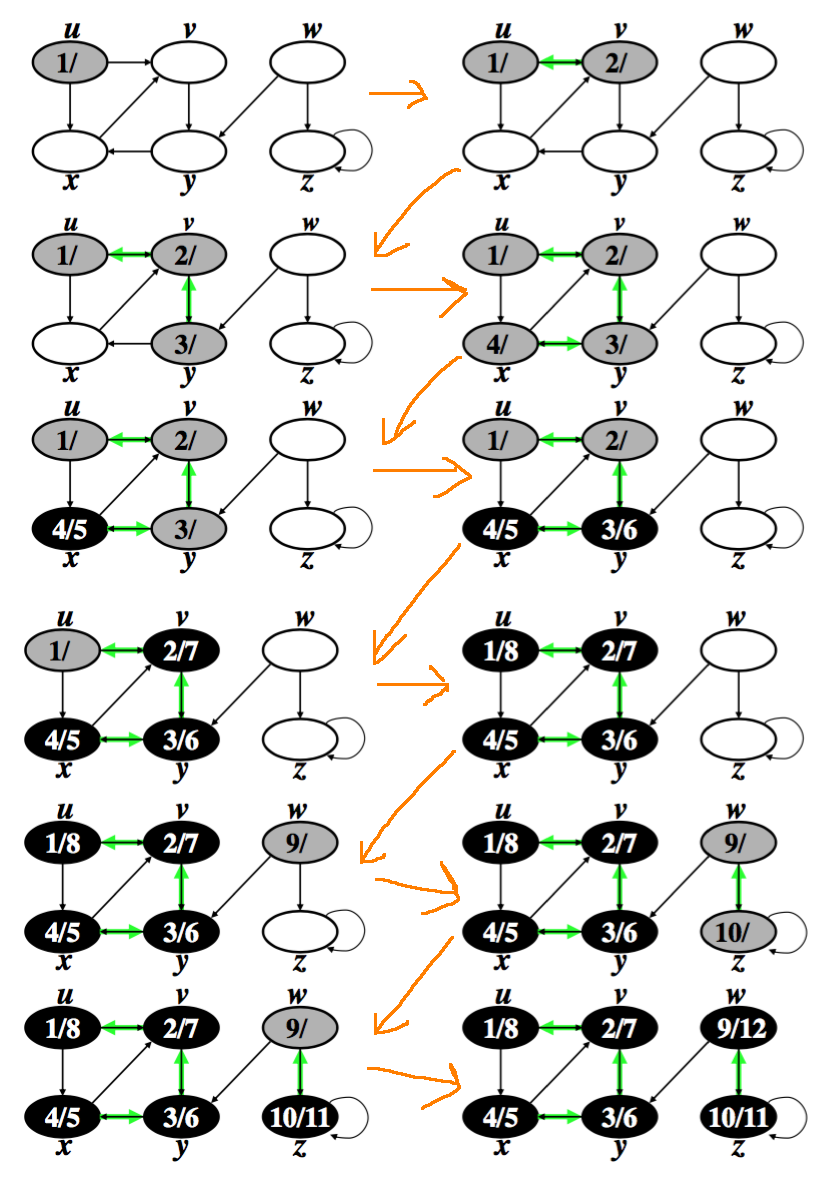
\includegraphics[width=.7\textwidth]{./notes/immagini/l6-fig1.png}
	\caption{Esplorazione in profondità}
\end{figure}

\subsection{Complessità}\label{complessituxe0}

La procedura \textsc{DFS} viene eseguita \emph{O(n)} volte, allo stesso
modo \textsc{DFS-Visit} viene chiamata esattamente una volta per ogni
vertice e per ognuno di essi scorre la lista delle adiacenze e, dal
momento che il ciclo \texttt{for} viene eseguito per ogni nodo, si ha che la
complessità totale della visita in profondità è \emph{O(n+m)}.

\subsection{Proprietà di DFS}\label{proprietuxe0-di-dfs}

DFS ha varie proprietà interessanti.

\subsubsection{Proprietà delle
parentesi}\label{proprietuxe0-delle-parentesi}

Se si rappresenta la scoperta di ogni vertice \emph{u} con una
partentesi aperta $(_u$ e la terminazione con una partentesi chiusa
$_u)$, si ottiene una sequenza ben formata di parentesi.

Ovvero per ogni coppia di vertici \emph{u} e \emph{v}, si può verificare
solamente uno di 4 casi:

\begin{enumerate}
\item
  $(_u \: \ldots\: _u) \: \ldots \: (_v \:\ldots \:_v)$
\item
  $(_v  \: \ldots \: _v) \: \ldots \: (_u \:\ldots \:_u)$
\item
  $(_u \: \ldots \: (_v \: \ldots \:_v) \: \ldots \:_u)$
\item
  $(_v \: \ldots \: (_u \: \ldots \: _u)\: \ldots \:_v)$
\end{enumerate}

\paragraph{Dimostrazione}\label{dimostrazione}

Assumendo che venga scoperto prima \emph{u} di \emph{v}, ovvero
$u.d < v.d$, si ha che, se $u.f < v.d$,
allora si verifica il caso 1.

Se invece $u.f > v.d$, allora quando \emph{v} viene
scoperto, \emph{u} è grigio, ovvero lo si sta ancora esplorando e
siccome il vertice \emph{v} è stato scoperto dopo, la sua lista della
adiacenze verrà esplorata completamente prima di quella del nodo
\emph{u}, si verifica quindi il caso 3.

I casi 2 e 4 sono simmetrici.

\subsubsection{Proprietà dei discendenti}\label{proprietuxe0-dei-discendenti}

Il vertice \emph{v} è discendente del vertice \emph{u} in un albero
della foresta di ricerca se e solo se $(_u \: \ldots \: (_v \: \ldots \:_v) \: \ldots \:_u)$.

\paragraph{Dimostrazione}\label{dimostrazione-1}

\emph{v} diventa un discendente solamente se viene scoperto dopo che è
stato scoperto il vertice \emph{u} e pertanto, verrà completata prima la
lista delle adiacenze di \emph{v} e poi quella di \emph{u}, pertanto per
la proprietà delle parentesi si ha che $(_u \: \ldots \: (_v \: \ldots \:_v) \: \ldots \:_u)$.

\subsubsection{Proprietà del cammino bianco}\label{proprietuxe0-del-cammino-bianco}

Se c'è un arco \emph{uv} e si sta espandendo il nodo \emph{u}, può
essere che il nodo \emph{v} sia già stato visitato perché la ricerca è
partita da un altro nodo \emph{w} ed è già stato trovato un cammino tra
\emph{w} e \emph{v}.

Quindi, il vertice \emph{v} diventa discendente del vertice \emph{u} in
un albero della foresta di visita in profondità se e solo se
nell'instante in cui \emph{u} viene scoperto esiste un cammino da
\emph{u} a \emph{v} i cui vertici sono tutti bianchi.

\paragraph{Dimostrazione}\label{dimostrazione-2}

Sia \emph{v} discendente di \emph{u}, ovvero c'è un cammino $u = x_0, x_1, \ldots, x_k = v$ nel ramo dell'albero della foresta di ricerca
che connette \emph{u} a \emph{v}.

Siccome $x_{i+1}$ viene scoperto visitando la lista delle adiacenze di
$x_i$, esiste l'arco $x_ix_{i+1}$ e inoltre $x_i$ viene
scoperto prima di $x_{i+1}$.

Quindi $u = x_0, x_1,\ldots,x_k = v$ è un cammino tale che quando
$u = x_0$ viene scoperto i vertici $x_1,\ldots,x_k = v$ non
sono ancora stati scoperti e dunque sono bianchi.

Supponendo il contrario, ovvero che quando \emph{u} viene scoperto
esiste un cammino bianco da \emph{u} a \emph{v}.

Siccome \emph{v} viene scoperto dopo di \emph{u}, per la proprietà delle
parentesi si ha che  $(_u \: \ldots\: _u) \: \ldots \: (_v \:\ldots \:_v)$ oppure
$(_u \: \ldots \: (_v \: \ldots \:_v) \: \ldots \:_u)$.

Se si verifica il secondo caso, allora \emph{v} è discendente di
\emph{u} per la proprietà dei discendenti.

Il primo caso invece non può accedere, perché, se per assurdo questo
succede, viene violata la proprietà delle parentesi. 
Sia \emph{w} il penultimo vertice del cammino bianco, ovvero il vertice $x_{k-1}$ che
è discendente di \emph{u} e connesso a \emph{v}. Per la proprietà delle
parentesi si ha $(_u \: \ldots \: (_w \: \ldots \: (_v \: \ldots\: _v) \: \ldots \: _w) \: \ldots \: _u)$ mentre secondo l'ipotesi dovrebbe essere 
$(_u \: \ldots \: (_w \: \ldots \: _w) \: \ldots \: _u) \: \ldots \: (_v \: \ldots\: _v)$ che è
assurdo.

\textbf{NB:} l'esistenza di un cammino bianco non implica che lo stesso
cammino sarà presente nell'albero dalla foresta.

\subsubsection{Classificazione degli archi}\label{classificazione-degli-archi}

Con la visita in profondità si possono classificare gli archi in 4
categorie:

\begin{enumerate}
\item
  \textbf{Archi d'albero}: archi \emph{uv} che connettono un padre ad un
  figlio in uno degli alberi, ovvero con \emph{v} scoperto visitando le
  adiacenze di \emph{u}.
\item
  \textbf{Archi all'indietro}: archi che connettono un nodo ad un suo
  predecessore nell'albero di ricerca, ovvero archi \emph{uv} con
  \emph{u=v} oppure \emph{v} ascendente di \emph{u} in un albero della
  foresta di ricerca.
\item
  \textbf{Archi in avanti}: archi che connettono un vertice ad un suo
  discendente, ovvero archi \emph{uv} con \emph{v} discendente di
  \emph{u} in un albero della foresta. Sia i cappi, che gli archi
  d'albero sono archi in avanti.
\item
  \textbf{Archi trasversali}: archi che connettono due vertici che si
  trovano in due rami distinti di un albero, ovvero archi \emph{uv} in
  cui \emph{v} ed \emph{u} appartengono a rami o alberi distinti della
  foresta.
\end{enumerate}

Da notare che lo stesso arco può appartenere a più categorie, in questo
caso gli si assegna la categoria nell'ordine in cui sono state
riportate.

\begin{figure}[htbp]
	\centering
	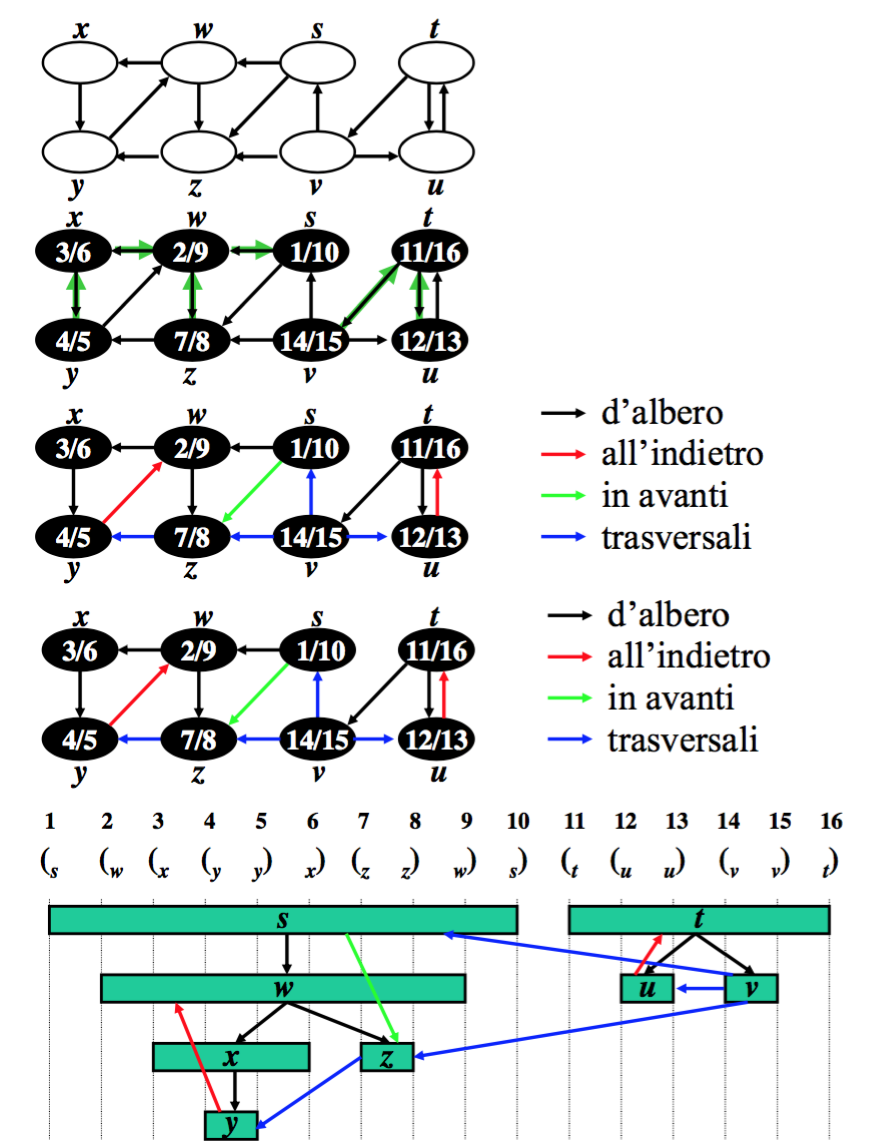
\includegraphics[width=.7\textwidth]{./notes/immagini/l6-fig2.png}
	\caption{Esplorazioni in profondità con categorizzazione degli archi e rappresentazione grafica delle parentesi}
\end{figure}

La classificazione degli archi può essere fatta durante la visita
dell'albero, andando a modificare la procedura \textsc{DFS-Visit}:

\begin{breakablealgorithm}
	\caption{DFS-Visit: versione con classificazione degli archi}
	\begin{algorithmic}[1]
		\Function{DFS-Visit}{u}
			\State $ time \gets time + 1 $
			\State $ u.d \gets time $
			\State $ u.color \gets grigio $
			\For{$ \forall v \in Adj[u] $}
				\If{$ v.color = bianco $}
					\State $(uv).tipo \gets albero$ \Comment{Il nodo viene scoperto da un arco diretto}
					\State $ v.\pi = u $
					\State \textsc{DFS-Visit}$ (v) $  \Comment{Visita in profondità dei vertici raggiungibili dal nodo}
				\EndIf
				\If{$ v.color = grigio $}
					\State $(uv).tipo \gets indietro$ \Comment{Vuol dire che il nodo è già stato scoperto e non è stato concluso, quindi è un discendente nel cammino corrente}
				\EndIf
				\If{$ v.color = nero $}
					\If{$ u.d < v.d $}
						\State $ (uv).tipo = avanti  $ \Comment{\textit{u} è stato scoperto prima di \textit{v}, quindi per la proprietà delle parentesi è un suo discendente, tuttavia la scoperta è avvenuta con un altro cammino, quindi l'arco uv è un arco in avanti}
					\EndIf
					\If{$ u.d > v.d $}
					\State $ (uv).tipo = trasversale  $ \Comment{il nodo \textit{v} è stato scoperto prima di \textit{u} ed è già stato chiuso, quindi si trova su un altro ramo o albero} 
					\EndIf
				\EndIf
			\EndFor
			\State $ time \gets time + 1 $
			\State $ u.f \gets time $
			\State $ u.color \gets nero $
		\EndFunction
	\end{algorithmic}
\end{breakablealgorithm}

\subsubsection{Visita in profondità su grafi orientati}\label{visita-in-profondituxe0-su-grafi-orientati}

Se il grafo sul quale viene effettuata la visita in profondità è
orientato possono essere presenti solamente archi d'albero e archi
all'indietro.

\todo[inline]{Integrare con registrazione}

Si può sfruttare questa proprietà per verificare la presenza di un ciclo
in un grafo orientato. Se durante la visita in profondità viene trovato
un arco all'indietro, vuol dire che c'è un ciclo. Questo risulta
efficiente perché in una foresta con \emph{d} alberi su \emph{n} nodi,
ci sono \emph{n-d} archi, ottenendo così una complessità \emph{O(n)}.

È ovvio che se viene trovato un arco all'indietro c'è un ciclo
nell'albero, ma la dimostrazione del contrario risulta meno ovvia:
supponendo che ci sia un ciclo e che il primo vertice del ciclo scoperto
sia il vertice \emph{u}. Gli altri nodi che compaiono del ciclo saranno
quindi bianchi e la visita in profondità andrà a visitare tutti i nodi
del ciclo, colorandoli. Quando la visita del ciclo sarà finita, il nodo
\emph{u} si avrà ancora un arco che lo collega all'ultimo nodo del ciclo
che è stato visitato e questo sarà un arco all'indietro.

\todo[inline]{Aggiungere esercizio 8, dalla registrazione}

\textbf{Provare esercizio 9 e 10}
